\documentclass[a4paper,11pt]{article}

% Identificação
\newcommand{\pbtitulo}{Hive}
\newcommand{\pbversao}{1.03}

\usepackage{../../sty/tutorial}

%----------------------------------------------------------------------
% Início do Documento
%----------------------------------------------------------------------
\begin{document}
	
	\maketitle % mostrar o título
	\thispagestyle{fancy} % habilitar o cabeçalho/rodapé das páginas
	
%--------------------------------------------------------------------------
% RESUMO DO ARTIGO
%--------------------------------------------------------------------------
\begin{abstract}
	% O primeiro caractere deve vir com \initial{}
	\initial{H}ive\cite{hiveoficial} ou "Apache Hive" (aqui chamarei apenas de Hive) é parte do Ecosistema Hadoop criado para ser um sistema de \textit{Data Warehouse} que é usado para analisar dados estruturados. Foi construído no topo do Hadoop e desenvolvido pelo Facebook. Como resultado, o Hive está intimamente integrado ao Hadoop e foi projetado para funcionar rapidamente em petabytes de dados. O que torna único é a capacidade de consultar grandes conjuntos de dados, aproveitando Apache Tez ou MapReduce, com uma interface semelhante a SQL. 
\end{abstract}

%--------------------------------------------------------------------------
% CONTEÚDO DO ARTIGO
%--------------------------------------------------------------------------
\section{Parte inicial}
O Hive fornece a funcionalidade de leitura, gravação e gerenciamento de grandes conjuntos de dados que residem em armazenamento distribuído. Executa linguagem semelhantes ao SQL padrão como consultas chamadas HQL (Hive query language) que são convertidas internamente em trabalhos MapReduce. Usar o Hive significa que podemos pular o requisito da abordagem tradicional de escrever programas MapReduce complexos. O Hive suporta linguagem de definição de dados (DDL), linguagem de manipulação de dados (DML) e funções definidas pelo usuário (UDF).  

\begin{figure}[H]
	\centering
	
\includegraphics[width=0.3\textwidth]{imagem/logo}
	\caption{Logo do Apache Hive}
\end{figure}

O Hive permite que você projete estrutura em grandes volumes de dados sem estrutura. Depois de definir a estrutura, você pode usar o HiveQL para consultar os dados sem conhecimento de Java ou do MapReduce. Também fornece suporte a serializador/desserializadores (SerDe) personalizados para dados complexos ou com estrutura irregular.

Há dois tipos de tabelas que você pode criar com o Hive:
\begin{itemize}
	\item \textit{Interna}: os dados são armazenados no data warehouse do Hive. O data warehouse está localizado no /hive/warehouse/ no armazenamento padrão para o cluster. São usadas nas seguintes condições:
	\begin{itemize}
		\item Os dados são temporários.
		\item Deseja que o Hive gerencie o ciclo de vida da tabela e dos dados.
	\end{itemize}
	\item \textit{Externa}: os dados são armazenados fora do data warehouse. Os dados podem ser guardados em qualquer armazenamento acessível pelo cluster. São usadas nas seguintes condições:
   	\begin{itemize}
   		\item Os dados também são usados fora do Hive. Por exemplo, os arquivos de dados são atualizados por outro processo (que não bloqueia os arquivos.)
   		\item Os dados devem permanecer no local anterior, mesmo depois de descartar a tabela.
   		\item Você precisa de um local personalizado, como uma conta de armazenamento não padrão.
   		\item Um programa que não seja o hive gerencia o formato de dados, local e assim por diante.
    \end{itemize}
\end{itemize}

\section{Arquitetura do Hive}
A seguinte imagem explica como se comporta o fluxo de envio de consulta no Hive:
\begin{figure}[H]
	\centering
	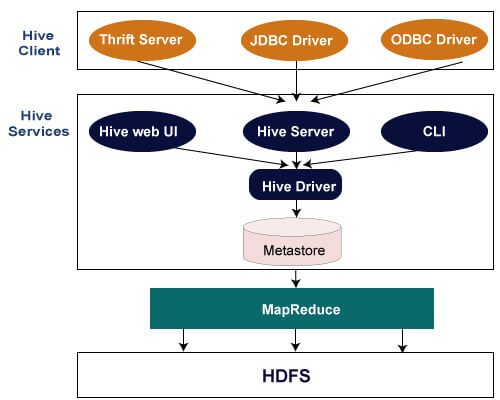
\includegraphics[width=0.7\textwidth]{imagem/architecture.jpg}
	\caption{Arquitetura do Apache Hive}
\end{figure}

Na primeira parte do \textit{Hive Client} significa que este permite escrever aplicativos em várias linguagens, incluindo Java, Python e C++. Ele suporta diferentes tipos de clientes, como:
\begin{itemize}
	\item \textit{Thrift Server} - É uma plataforma de provedor de serviços multilíngue que atende a solicitação de todas as linguagens de programação que suportam o Thrift.
	\item \textit{Driver JDBC} - É usado para estabelecer uma conexão entre o hive e os aplicativos Java. O Driver JDBC está presente na classe org.apache.hadoop.hive.jdbc.HiveDriver.
	\item \textit{Driver ODBC} - Permite que os aplicativos que suportam o protocolo ODBC se conectem ao Hive. 
\end{itemize}

Na segunda parte do \textit{Hive Services} temos:
\begin{itemize}
	\item \textit{Hive Web UI} (Interface de usuário da Web do Hive) - é uma alternativa da CLI do Hive. Fornece uma GUI baseada na Web para executar consultas e comandos do Hive.
	\item \textit{Hive Server} - É referido como Apache Thrift Server. Aceita a solicitação de diferentes clientes e a fornece ao Hive Driver.
	\item \textit{Hive CLI} (Command Line Interface) - É um shell onde podemos executar consultas e comandos do Hive.
	\item \textit{Hive Driver} - Recebe consultas de diferentes fontes, como UI da web, CLI, Thrift e driver JDBC/ODBC. Transfere as consultas para o compilador.
	\item \textit{Hive MetaStore} - Repositório central que armazena todas as informações de estrutura de várias tabelas e partições do \textit{WareHouse}. Também inclui os metadados das colunas e suas informações, serializadores e desserializadores pode ser usados para ler e gravar dados e nos arquivos HDFS correspondentes onde os dados são armazenados.
\end{itemize}

Temos ainda duas ferramentas destinadas a suportar essa camada: 
\begin{itemize}
	\item \textit{Hive Compiler} - O objetivo do compilador é analisar a consulta e realizar análise semântica nos diferentes blocos e expressões de consulta. Ele converte instruções HiveQL em trabalhos MapReduce.
	\item \textit{Hive Execution Engine} - Otimizador responsável por gerar um plano lógico na forma de DAG de tarefas de redução de mapa e tarefas HDFS. No final, o mecanismo de execução executa as tarefas recebidas na ordem de suas dependências. 
\end{itemize}

\section{Hadoop no Docker}
O modo mais simples de se conseguir trabalhar com o Hadoop é utilizando o Docker, para baixar a imagem do Hadoop: \\
\codigo{\$ docker pull suhothayan/hadoop-spark-pig-hive:2.9.2}

Nessa imagem temos outros produtos do Ecossistema Hadoop: Spark, Pig e Hive. Para criar e executar a primeira vez o contêiner (a pasta que este comando for executado será associada a uma pasta interna chamada \textbf{/home/tsthadoop}): \\
\codigo{\$ docker run -it -d --name meu-hadoop -v \$(pwd):/home/tsthadoop \\ suhothayan/hadoop-spark-pig-hive:2.9.2}

Uma vez interrompido o contêiner: \\
\codigo{\$ docker stop meu-hadoop}

Podemos executá-lo novamente com os seguintes comandos: \\
\codigo{\$ docker start meu-hadoop \\
\$ docker exec -it meu-hadoop /etc/bootstrap.sh bash}

\subsection{Erro de Permissão}
Na primeira vez que entramos é dado um erro na execução do script "bootstrap.sh" de permissão negada para executar o script "spark-env.sh", vamos corrigir isso com o comando: \\
\codigo{\# chmod 777 /usr/local/spark/conf/spark-env.sh}

Vamos sair do bash: \\
\codigo{\# exit}

Podemos executá-lo novamente: \\
\codigo{\$ docker exec -it meu-hadoop /etc/bootstrap.sh bash}

E o erro desapareceu.


E podemos verificar a versão do Hadoop e Hive que estão instalados: \\
\codigo{\$ hadoop version \\
\ttfamily\$ hive --version}

O endereço da pasta do Hive: \\
\codigo{\$ cd /usr/local/hive}

\section{Uma pasta para seus Dados}
Observe que no comando de criação do contêiner foi associada uma pasta (que é a pasta atual) com uma pasta interna deste, então por exemplo, se estamos na pasta "/Aplicativos/hadoop-model" e iniciamos o contêiner essa pasta estará associada.

No caso do Hive este cria uma pasta chamada "metastore\_db" e isso pode ser um problema, pois se mudamos de pasta o Hive pode até mesmo não iniciar, então na primeira vez que executar o Hive tenha a certeza da pasta que se encontra.

E inclusive não se esqueça de sempre estar na pasta associada quando for iniciar o Hive: \\
\codigo{\# cd /home/tsthadoop/} \\
\codigo{\# hive}

\subsection{Se caso der problema?}
Pode acontecer dessa pasta se corromper, aí não temos outra saída a não ser recriar a pasta, remova esta do diretório: \\
\codigo{\# rm -rf metastore\_db}

Recriá-la com o comando: \\
\codigo{\# schematool -dbType derby -initSchema}

Isso mesmo que percebemos isso é uma pasta do banco "Apache Derby".

\section{Comando SQL}
O Hive trabalha essencialmente com comandos "similares" aos do SQL, vamos começar olhando quais são as bases existentes: \\
\codigo{hive> show databases;}

Criar uma nova base de dados: \\
\codigo{hive> create database amostra;}

Entrar nessa base de dados: \\
\codigo{hive> use amostra;}

Verificar as tabelas existentes: \\
\codigo{hive> show tables;}

\subsection{Buscar dados do Hadoop}
Agora vamos brincar um pouco da integração entre o Hive e o Hadoop, para isso existe um arquivo chamado "201808\_BF\_Amostra.csv" que deve ser adicionado ao HDFS, para isso, saimos do Hive: \\
\codigo{hive> exit;}

Adicionar os arquivos no HDFS: \\
\codigo{\# hadoop fs -put 201808\_BF\_Amostra.csv}

Retornamos ao hive: \\
\codigo{\# hive}

E entre novamente no database que criamos: \\
\codigo{hive> use amostra;}

Não é por escolha minha, mas infelizmente todos os campos dessa base são do tipo String, foram todos colocados em aspas duplas, então como desejo apenas testar a funcionalidade vamos criar todos os campos da tabela assim: \\
\codigo{hive> create table amostra2018 (anoPag string, ano2 string, estado string, \\ cod string, cidade string, cpf string, nome string, valor string) ROW FORMAT \\ DELIMITED FIELDS TERMINATED BY ';';}

O comando SQL é basicamente a mesma coisa o final é que existem algumas palavras chaves indicando para o Hive como deve se comportar, para importarmos os dados: \\
\codigo{hive> LOAD DATA INPATH '201808\_BF\_Amostra.csv' into table amostra2018;}

Podemos verificar os dados com: \\
\codigo{hive> select * from amostra2018 limit 10;}

Ou sem usar a cláusula limit para vermos todos. Agora o mais interessante é, saia do Hive e digitar o comando: \\
\codigo{\# hadoop fs -ls}

E descobrimos que o arquivo "sumiu" do HDFS, pois o Hive disse para o Hadoop: "Ele agora é meu!". E ficou com a guarda do arquivo.

\subsection{Inserir Dados}
Vamos criar um novo Database: \\
\codigo{hive> create database novo;}

Acessar este Database: \\
\codigo{hive> use novo;}

Criar uma tabela: \\
\codigo{hive> create table teste (codigo int, nome string) ROW FORMAT DELIMITED \\
FIELDS TERMINATED BY ',';}

E inserir alguns dados nela: \\
\codigo{hive> insert into table teste \\ 
values(123, 'Fernando Anselmo'),(456, 'Maria Claudia')}

Neste momento vemos que o processo é basicamente similar a obter os dados do HDFS. Realizando um Map/Reduce automático para adicionar os dados a tabela. Podemos verificar seu conteúdo. \\
\codigo{hive> select * from teste;}

Basicamente todas as funcionalidades do comnando SELECT do SQL estão a disposição do Hive. Como por exemplo: \\
\codigo{hive> select * from teste where nome like '\%Anselmo';}

Conceito de chave primária não existe aqui, assim ao dispararmos novamente o comando: \\
\codigo{hive> insert into table teste values(123, 'Fernando Anselmo');}

Temos mais um registro com o código igual a 123 e o nome igual a 'Fernando Anselmo'.

\section{Acesso via JDBC}
Nada disso teria graça senão usássemos Java para demonstrar as ligações do Hive, para isso vamos utilizar o Spring Tool Suite no qual criamos um projeto \textit{Maven Project}. Só que antes de fazermos isso precisamos configurar algumas questões de segurança.

Primeiro precisamos saber qual o nosso hostname: \\
\codigo{\# hostname}

Anote esse número (que é o CONTEINER ID), de posse deste, vamos editar o arquivo \textbf{core-site.xml.template} do Hadoop com o seguinte comando: \\
\codigo{\# vim \$HADOOP\_PREFIX/etc/hadoop/core-site.xml.template}

Adicionar as seguintes propriedades:
\begin{lstlisting}[]
  <property>
    <name>hadoop.proxyuser.root.hosts</name>
    <value>*</value>
  </property>
  <property>
    <name>hadoop.proxyuser.root.groups</name>
    <value>*</value>
  </property>
  <property>
    <name>hive.execution.engine</name>
    <value>spark</value>
  </property>  
\end{lstlisting}

Para salvar pressione ESC e digite \textbf{:wq}. Essas configurações permitem que o usuário root consiga atravessar o proxy do Hadoop e acessar o Hive. Sair da imagem, parar e iniciar o contêiner, entrar no bash novamente.

Agora precisamos ativar o serviço do Hive para permitir a conexão: \\
\codigo{\# hive --service hiveserver2 \&}

Quando terminar de processar basta dar Enter para retornar ao terminal e podemos testar se está funcionando com o comando \textbf{beeline}: \\
\codigo{\# beeline -u jdbc:hive2://[hostname]:10000/ -n root}

Que deve entrar no bash do Hive, e damos o comando: 
\codigo{dbc:hive2://[hostname]:10000/> show databases;}

Para verificarmos as bases de dados ativas e receberemos a \textbf{default}. E agora estamos prontos.

A grande vantagem de criarmos um projeto tipo Maven que podemos inserir todas as bibliotecas que necessitamos sem termos o menor trabalho, basta apenas buscamos estas do repositório central do Maven através de sua declaração no arquivo \textbf{pom.xml}:
\begin{lstlisting}[]
<project xmlns="http://maven.apache.org/POM/4.0.0"
  xmlns:xsi="http://www.w3.org/2001/XMLSchema-instance"
  xsi:schemaLocation="http://maven.apache.org/POM/4.0.0 https://maven.apache.org/xsd/maven-4.0.0.xsd">
  <modelVersion>4.0.0</modelVersion>
  <groupId>hiveproj</groupId>
  <artifactId>hiveproj</artifactId>
  <version>0.0.1-SNAPSHOT</version>
  <name>Projeto em Hive</name>
  <description>Exemplo do projeto em Hive</description>
  <dependencies>
    <dependency>
      <groupId>org.apache.hive</groupId>
      <artifactId>hive-jdbc</artifactId>
      <version>2.3.5</version>
    </dependency>
    <dependency>
      <groupId>org.apache.hadoop</groupId>
      <artifactId>hadoop-common</artifactId>
      <version>2.9.2</version>
    </dependency>
  </dependencies>
</project>
\end{lstlisting}

Assim de forma simples temos as bibliotecas do Hive. Vamos começar com uma classe que além de testar nossa conexão criará uma tabela:
\begin{lstlisting}[]
package hiveproj;

import java.sql.Connection;
import java.sql.DriverManager;
import java.sql.ResultSet;
import java.sql.SQLException;
import java.sql.Statement;

public class HiveTeste {
  private static String driverName = "org.apache.hive.jdbc.HiveDriver";

  public static void main(String[] args) throws SQLException {
    try{
      Class.forName(driverName);
    } catch (ClassNotFoundException e) {
      e.printStackTrace();
      System.exit(1);
    }

    Connection con = DriverManager.getConnection("jdbc:hive2://172.17.0.2:10000/default", "root", "");
    Statement stmt = con.createStatement();
    String tableName = "HiveByJava";
    stmt.execute("drop table if exists " + tableName);
    stmt.execute("create table " + tableName +
      " (key int, value string) ROW FORMAT DELIMITED FIELDS TERMINATED BY \",\"");
    System.out.println("Tabela criada com sucesso!");

    String sql = "show tables";
    System.out.println("Executando: " + sql);
    ResultSet res = stmt.executeQuery(sql);
    if (res.next()) {
       System.out.println(res.getString(1));
    }

    sql = "describe " + tableName;
    System.out.println("Executando: " + sql);
    res = stmt.executeQuery(sql);
    while (res.next()) {
      System.out.println(res.getString(1) + "\t" + res.getString(2));
    }

    System.out.println("Tabela criada sem problemas");
  }
}
\end{lstlisting}

Não pretendo ficar "enchendo linguiça" nessa apostila mostrando o que é possível realizar com uma conexão JDBC (para isso inclusive tenho meu primeiro livro de Java escrito), mas uma dica, não realizar comandos de inserção pois o Hive não gosta muito deles e tem que acertar várias bases. Então se precisar inserir dados na tabela use a técnica mostrada no início.

Mais fontes de informação podem ser obtidas em diversos sites que apresenta tutoriais completos sobre o Apache Hive como a Tutorials Point\cite{tutorialspoint}.
	
\section{Conclusão}
Hive é um sistema de armazenamento de dados distribuído e tolerante a falhas que permite análises de dados em grande escala. Um data warehouse fornece um armazenamento central de informações que podem ser facilmente analisadas para tomar decisões informadas e orientadas por dados. Permite que os usuários leiam, gravem e gerenciem petabytes de dados usando SQL. 

Hive foi criado para permitir que não programadores familiarizados com SQL trabalhem com petabytes de dados, usando uma interface semelhante a SQL chamada HiveQL. Os bancos de dados relacionais tradicionais são projetados para consultas interativas em conjuntos de dados pequenos e médios e não processam bem conjuntos de dados enormes. Em vez disso, usa processamento em lote para funcionar rapidamente em um banco de dados distribuído muito grande. 

Hive transforma as consultas HiveQL em trabalhos MapReduce ou Apache Tez que são executados na estrutura de agendamento de trabalho distribuído do Apache Hadoop ou do YARN (\textit{Yet Another Resource Negotiator}). Consulta dados armazenados em uma solução de armazenamento distribuído, como o HDFS (\textit{Hadoop Distributed File System}) ou o Amazon S3. Armazena seus metadados de banco de dados e tabela em um metastore, que é um banco de dados ou armazenamento com suporte de arquivo que permite fácil abstração e descoberta de dados. 

Sou um entusiasta do mundo \textbf{Open Source} e novas tecnologias. Qual a diferença entre Livre e Open Source? \underline{Livre} significa que esta apostila é gratuita e pode ser compartilhada a vontade. \underline{Open Source} além de livre todos os arquivos que permitem a geração desta (chamados de arquivos fontes) devem ser disponibilizados para que qualquer pessoa possa modificar ao seu prazer, gerar novas, complementar ou fazer o que quiser. Os fontes da apostila (que foi produzida com o LaTex) está disponibilizado no GitHub \cite{github}. Veja ainda outros artigos que publico sobre tecnologia através do meu Blog Oficial \cite{fernandoanselmo}.

%--------------------------------------------------------------------------
% REFERÊNCIAS
%--------------------------------------------------------------------------
\begin{thebibliography}{4}
	\bibitem{hiveoficial} 
	Página do Apache Hive \\
	\url{https://hive.apache.org/}

	\bibitem{tutorialspoint} 
	Tutorials Point sobre Hive \\
	\url{https://www.tutorialspoint.com/hive/index.htm}
	
		\bibitem{fernandoanselmo} 
	Fernando Anselmo - Blog Oficial de Tecnologia \\
	\url{http://www.fernandoanselmo.blogspot.com.br/}
	
	\bibitem{publicacao} 
	Encontre essa e outras publicações em \\
	\url{https://cetrex.academia.edu/FernandoAnselmo}
	
	\bibitem{github} 
	Repositório para os fontes da apostila \\
	\url{https://github.com/fernandoans/publicacoes}
\end{thebibliography}

\end{document}